%!TEX root = ../report.tex

\begin{document}
    \chapter{Methodology}
        In this section, a brief description of the Data and the definition of the Registration Problem will be given.
        The structure of a CityGML model is complex, and their complete explanation is out of the scope of this project,
        For detailed information about CityGML please refer to Gröger et. al \cite{Groger_2012_OGC} or the official websites.

%-------------------------------------------------------------------------------
%	Data
%-------------------------------------------------------------------------------
    \section{Data}   
        The CityGML models are public data in some states in Germany, for example in Nordrhein-Westfalen \cite{NRW3DModel_online}. 
        Other states of Germany like Hessen \cite{Hessen3DModel_online} or Bayern \cite{Bayern3DModel_online} charge money for their Models.
        That is not relevant for this project because the CityGML Models are received from the server of the A-DRZ project.

        Besides the representation of the building, CityGML models provide other interesting information about the buildings.
        For this work, the intersection of the model with the terrain is the most relevant information.
        The terrain intersection is provided as an array of 3D points that represent some points on the walls that intersect with the
        ground. 
        
        The point cloud data is collected and provided by the A-DRZ project partners that develop and operate the actual Robots.
        These are mainly the University of Bonn \cite{UniBonn_online} and the Technical University of Darmstadt \cite{TUDarmstadt_online},
        which have integrated corresponding laser scanners and Lidar sensors on their platforms.

        \autoref{fig:initial_front_model} and \autoref{fig:initial_back_model} show a CityGML model and its corresponding point cloud
        before being registered.
            
        Unfortunately, there is no ground truth for the registration of the data available. 
        Therefore, the results are evaluated manually by a person who decides whether the registration was successful or not.

        \begin{figure}[H]
            \centering
            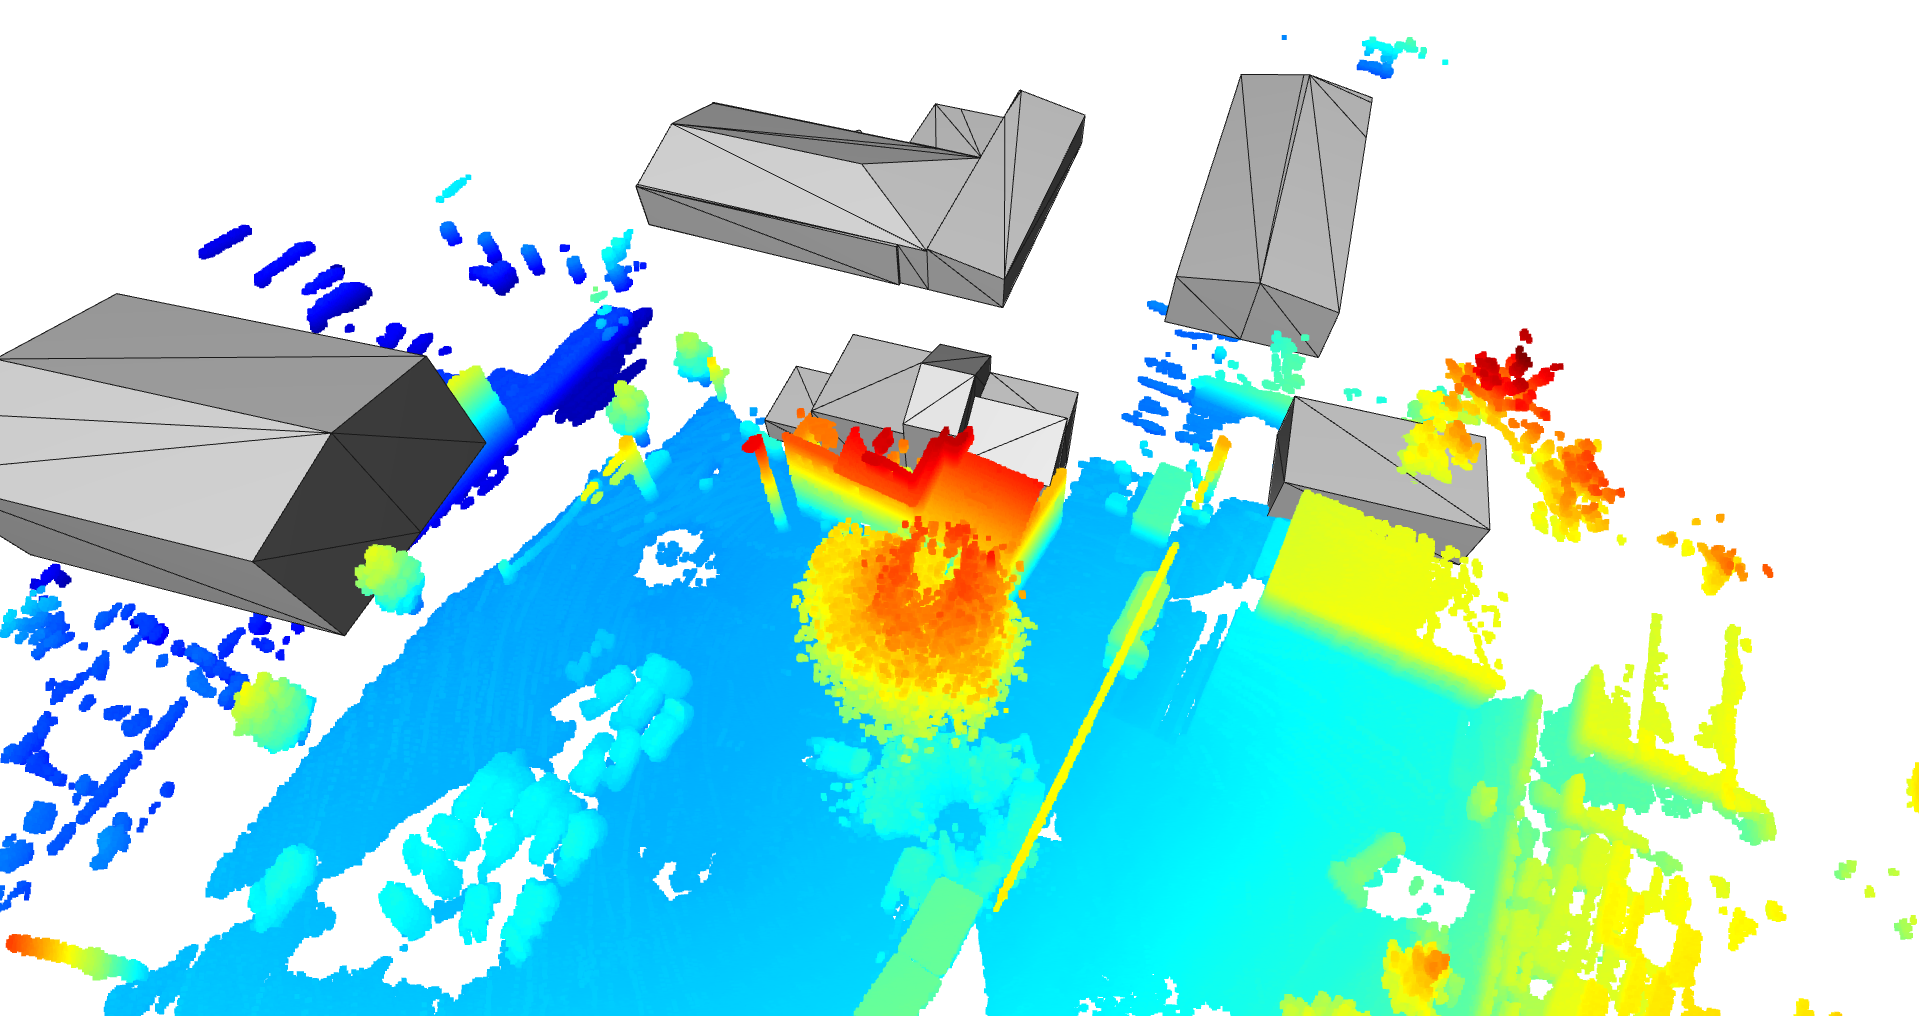
\includegraphics[scale=0.2]{images/solution_images/initial_front_model.png}
            \caption{Front view of a point cloud and a model before registration.}
            \label{fig:initial_front_model}
        \end{figure}
      
        \begin{figure}[H]
            \centering
            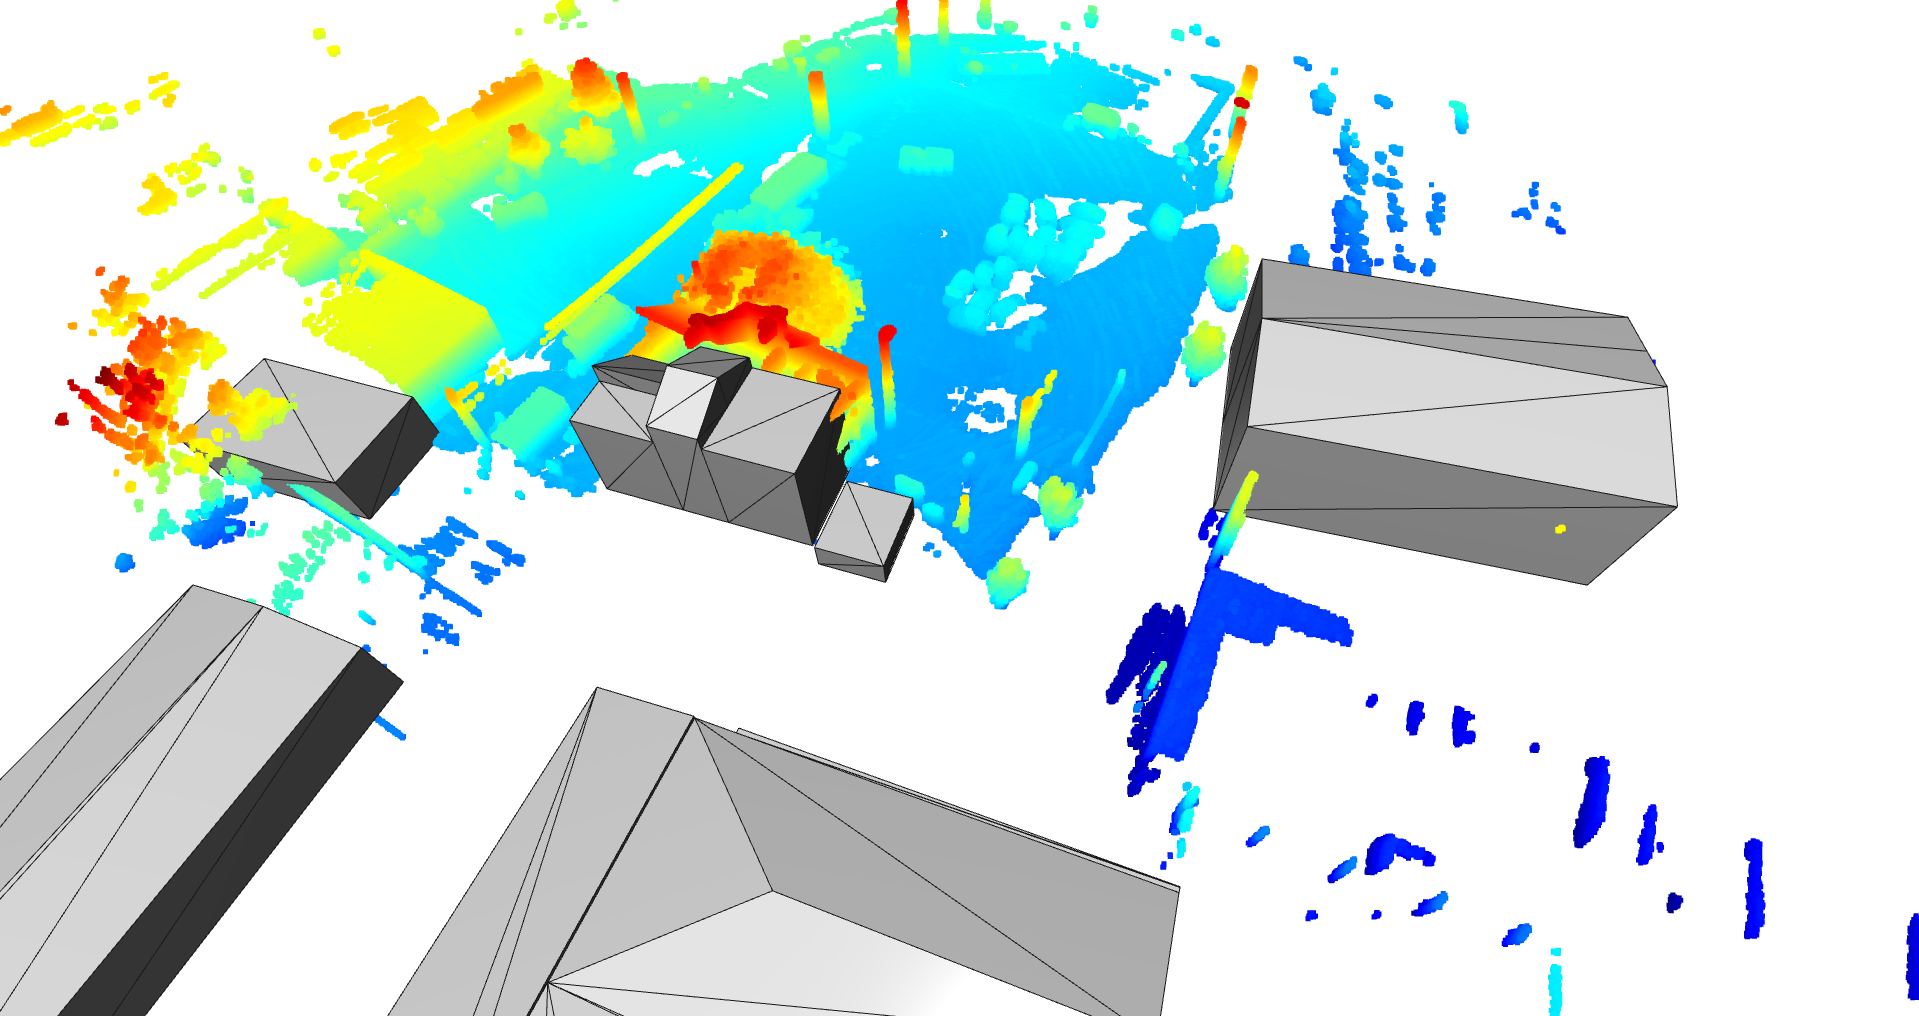
\includegraphics[scale=0.2]{images/solution_images/initial_back_model.png}
            \caption{Back view of a point cloud and a model before registration.}
            \label{fig:initial_back_model}
        \end{figure}
        
        

        % \begin{figure}
        %     \begin{subfigure}{0.49\textwidth}
        %       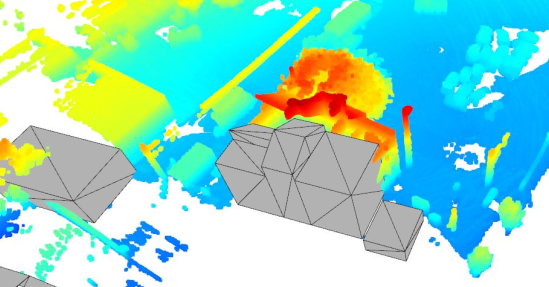
\includegraphics[width=\linewidth]{images/solution_images/initial_back_model_zoom.png}
        %       \caption{Model as mesh.} \label{fig:initial_back_zoom_a}
        %     \end{subfigure}%
        %     \hspace*{\fill}   % maximize separation between the subfigures
        %     \begin{subfigure}{0.49\textwidth}
        %       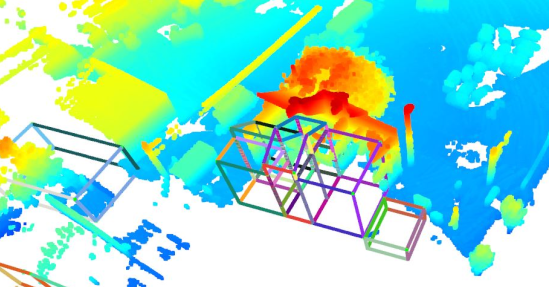
\includegraphics[width=\linewidth]{images/solution_images/initial_back_lines_zoom.png}
        %       \caption{Edges of the model as set of points.} \label{fig:initial_back_zoom_b}
        %     \end{subfigure}%
        %     \hspace*{\fill}   % maximizeseparation between the subfigures
        %   \caption{Zoom into the back view.} \label{fig:initial_back_zoom}
        % \end{figure}

%-------------------------------------------------------------------------------
%	Setup
%-------------------------------------------------------------------------------
    \section{Setup}
        The main setup is depicted in \autoref{fig:system_diagram}.
        The input of the system is a CityGML model and its corresponding point cloud. 
        The output of the registration algorithm is a transformation that aligns the point cloud with the CityGML model.
        This transformation is then used to visualize the alignment of the input data for its proper evaluation.

%-------------------------------------------------------------------------------
%	Registration Problem in 3D
%-------------------------------------------------------------------------------
    \section{Registration Problem in 3D}
    \label{section:Registration Problem in 3D}
        In general, the registration task consists of finding the transformation that aligns the input CityGML model with the input point cloud.

        More specifically, given a source point set $P = \{p_i\}_{i=1}^N$, where $p_i \in \mathbb {R}^{4}$,
        and a target point set $Q = \{q_j\}_{j=1}^M$, where $q_j \in \mathbb {R}^{4}$,
        the registration task consists of finding a transformation $T \in SE(3)$ that minimizes:
        \begin{equation}
            \label{eq:lossfunction}
            \sum_{i = 1}^{N} \min_{j \in {1...M}} d( T p_i , q_j )    
        \end{equation}
          
        where $d(T p_i, q_j)$ is the Euclidian distance between $H p_i$ and $q_j$.
        $p_i$ and $q_j$ are points in homogeneous coordinates. Therefore, their fourth element is $1$.

        In this case, the point set $P$ corresponds to the point cloud, while the point set $Q$ corresponds to the CityGML model.
        It is clear that $P$ is formed by the same points that form the point cloud, 
        but the set $Q$ could be a sampled point cloud from the CityGML model
        or other characteristic points of the CityGML model.
        
        The difficulty of this task is to find correspondences between $P$ and $Q$ that minimizes \autoref{eq:lossfunction}.
        If the correspondences were defined, the registration would be pretty straightforward and correct.

%-------------------------------------------------------------------------------
%	Registration Problem in 2D
%-------------------------------------------------------------------------------
    \section{Registration Problem in 2D}
    \label{section:Registration Problem in 2D}
        To simplify the problem, one can transform the 3D registration problem into a 2D registration problem 
        by projecting the point cloud and the CityGML model onto the xy-plane.

        The registration problem in 2D remains the same as in 3D, but $p_i \in \mathbb{R}^{3}$, $q_j \in \mathbb {R}^{3}$, and $T \in SE(2)$.
        Again, $p_i$ and $q_j$ are points in homogeneous coordinates and their third element is always $1$.

%-------------------------------------------------------------------------------
%	Registration Problem as Mixed Integer Linear Program
%-------------------------------------------------------------------------------
    \section{Registration Problem as Mixed Integer Linear Program}
    \label{section:Registration Problem as Mixed Integer Linear Program}
        The 3D registration problem defined in \autoref{section:Registration Problem in 3D} can be redefined as a Mixed Integer Linear Program.
        The exact definition is given in \cite{Sakakubara_2007_automatic}.

        The 2D registration problem defined in \autoref{section:Registration Problem in 2D} can be redefined as a Mixed Integer Linear Program in the same way.
        The objective is to maximize
        
        \begin{equation}
            \label{eq:objective_original}
            \sum_{i}^{N} \sum_{j}^{M} x_{ij}    
        \end{equation}
        
        subject to
        
        \begin{equation}
            \label{eq:subject_sum_rows}
            \sum_{i}^{N} x_{ij} \leq 1
        \end{equation}
        
        \begin{equation}
            \label{eq:subject_sum_columns}
            \sum_{j}^{M} x_{ij} \leq 1
        \end{equation}

        \begin{equation}
            \label{eq:subject_transformation_0}
            \sum_{i}^{N} \sum_{j}^{M} l_{0} \leq \epsilon_d + b (1 - x_{ij})
        \end{equation}

        \begin{equation}
            \label{eq:subject_transformation_negative_0}
            \sum_{i}^{N} \sum_{j}^{M} -l_{0} \leq \epsilon_d + b (1 - x_{ij})
        \end{equation}

        \begin{equation}
            \label{eq:subject_transformation_1}
            \sum_{i}^{N} \sum_{j}^{M} l_{1} \leq \epsilon_d + b (1 - x_{ij})
        \end{equation}

        \begin{equation}
            \label{eq:subject_transformation_negative_1}
            \sum_{i}^{N} \sum_{j}^{M} -l_{1} \leq \epsilon_d + b (1 - x_{ij})
        \end{equation}

        \begin{equation}
            \label{eq:subject_lines_preservation}
            \sum_{i}^{N} \sum_{k}^{N} \sum_{j}^{M} \sum_{l}^{M} x_{ij} + x_{kl} \leq 1 \;\;\; for \;\;\; \mid d(p_i, p_k) - d(q_j, q_l) \mid \geq \epsilon_l
        \end{equation}

        \begin{equation}
            \label{eq:subject_transformation_variables}
            \begin{gathered}
                \delta_1^- \leq t_{11} \leq \delta_1^+ \\
                \delta_2^- \leq t_{12} \leq \delta_2^+ \\
                t_x^- \leq t_{13} \leq t_x^+ \\
                t_y^- \leq t_{23} \leq t_y^+ \\
                t_{11} = t_{22} \\
                t_{21} = -t_{12}
            \end{gathered}
        \end{equation}
        

        $X \in \mathbb{R}^{N \times M}$ is the matrix that represents the correspondences.
        That means that $x_{ij} = 1$ if the point $p_i$ in the source image corresponds to the point $q_j$ in the target image, otherwise $x_{ij} = 0$.

        $L = (q_i - T p_i)$ and the constant $\epsilon_d$ is a threshold to remove outliers. 
        In other words, $\epsilon_d$ is the maximum distance allowed between a target point and its corresponding source point after transformation.

        The constant $b$ is some large number. For example, $b$ can be two times the maximum distance between points in the source and the target image.

        The \autoref{eq:subject_lines_preservation} is used to preserve lines between points after the transformation.
        If $\mid d(p_i, p_k) - d(q_j, q_l) \mid \geq \epsilon_l$, then either $p_i$ corresponds to $q_j$ or $p_k$ corresponds to $q_l$.
        The constant $\epsilon_l$ depends on $\epsilon_d$ and according to \cite{Sakakubara_2007_automatic}, 
        $\epsilon_l \geq 2 \sqrt{3} \epsilon_l$ needs to be satisfied because $\epsilon_d$ is the allowed rigid transformation error.

        The elements of $T$ are constrained in \autoref{eq:subject_transformation_variables},
        but the rest of the elemnts are constant: $t_{31} = 0$, $t_{32} = 0$, and $t_{33} = 1$.
        
          
\end{document}
